
今天所有的高性能計算機都有多個CPU或多個CPU內核(單個包中的獨立處理器)。大多數筆記本電腦至少有兩個內核,通常是四個。在性能的上下文中,高效程序不會讓任何硬件處於空閒狀態。如果程序只使用一小部分計算能力,例如:多個CPU內核中的一個,那麼就不是高效或高性能的。一個程序在同一時間使用多個處理器的方法,只有運行多個線程或進程。另外,這並不是使用多處理器的唯一方法,例如:很少有筆記本電腦用於高性能計算。相反,它們可以使用多個CPU來更好地同時運行不同且獨立的程序。這是一個非常好的模型,只是在高性能計算上下文中不是我們感興趣的那種。HPC系統通常會在每臺計算機上運行程序,甚至在分佈式計算的情況下在多臺計算機上運行同一個程序。那麼程序如何使用多個CPU?可以讓程序運行多個線程。

\subsubsubsection{5.2.1\hspace{0.2cm}線程是什麼?}

線程是一個指令序列,可以獨立於其他線程執行。多個線程可以在同一個程序中併發運行。所有線程共享相同的內存,相同進程的線程運行在同一臺機器上(HPC程序也可以包含多個進程)。分佈式程序可以運行在多臺機器上,並可以使用許多進程。分佈式計算的主題超出了本書的範圍,我們現在在瞭解如何最大化這些進程的性能。

那麼,多線程的性能有什麼可聊的呢?首先,只有當系統有足夠的資源,能夠同時執行多個指令序列時,同時執行多個指令序列才會讓性能更好。否則,操作系統需要在不同的線程之間切換,以確保每個線程都有時間片可以執行。

單個處理器上,忙於計算的線程提供儘可能多的工作讓處理器處理,即使線程沒有使用所有的計算單元或正在等待內存訪問,並且處理器一次只能執行一個指令序列-有一個程序計數器。現在,如果線程正在等待某些東西,比如用戶輸入或網絡信息,那麼CPU處於空閒狀態,可以執行另一個線程,而不會影響第一個線程的性能。這裡,操作系統會處理線程之間的切換。注意,等待內存並不算等待。當一個線程等待內存時,只是需要更長的時間來執行一條指令。當一個線程在等待I/O時,必須進行一個操作系統調用,然後該線程會被操作系統阻塞,直到操作系統喚醒才執行其他操作。

如果目標是提高程序的整體效率,那麼執行繁重計算的線程就需要有足夠的資源。考慮線程的資源時,想到的是使用多個處理器或處理器核心。也有其他方法,可以通過併發性來提高資源利用率,我們將看到這一點。

\subsubsubsection{5.2.2\hspace{0.2cm}對稱多線程}

處理器有很多計算硬件,大多數程序很少可以使用所有的硬件,程序中的數據依賴關係限制了處理器的計算能力。如果處理器有空閒的計算單元,就不能同時執行另一個線程來提高效率嗎?這就是\textbf{對稱多線程(SMT)}背後的思想,也稱為\textbf{超線程}。

支持SMT的處理器只有一組寄存器和計算單元,但是有兩個(或更多)程序計數器和一個計數器副本,用來維護正在運行的線程的狀態(具體的實現因處理器的不同而不同)。操作系統將單個處理器視為兩個(通常)或多個獨立處理器,每個處理器能夠運行一個線程。實際上,運行在一個CPU上的線程會競爭共享的資源,比如寄存器。如果每個線程沒有充分利用這些共享資源,SMT可以提供顯著的性能提高。換句話說,其通過運行多個這樣的線程來彌補一個線程的低效。

實際中,大多數支持SMT的處理器都可以運行兩個線程,而且性能的提高很多。很少看到100\%的加速(兩個線程都以全速運行),通常實際的加速在25\%到50\%之間(第二個線程實際上以四分之一到一半的速度運行),但是有些程序沒有加速。出於本書的目的,不會以任何特殊的方式對待SMT線程。對於程序來說,SMT處理器就像兩個處理器,在不同內核上運行的兩個線程性能情況,同樣適用於恰好在同一內核上運行的兩個線程的性能。這時,必須衡量運行的線程數是否大於物理內核數,並且是否能夠為程序提供加速,從而確定要運行多少個線程。

無論是共享整個物理核,還是SMT硬件創建的邏輯核,併發的性能在很大程度上取決於工作線程的獨立性。這是由算法和線程之間的工作劃分決定的,關於這兩個問題的書都有百本之多,但這個問題不在本書的討論範圍內。我們現在關注的是影響線程交互,並決定特定實現成功或失敗的因素。

\subsubsubsection{5.2.3\hspace{0.2cm}線程和內存}

由於多個線程之間對CPU進行時間切片不會帶來性能上的好處,所以在本章的其餘部分,假設在每個處理器核心上運行一個HPC線程(或者在由SMT處理器提供的每個邏輯核心上運行一個線程)。只要這些線程不競爭資源,就可以彼此獨立運行,程序就可以有加速。兩個線程在同一時間內完成的工作是一個線程的兩倍。如果工作可以在兩個線程之間,以一種獨立的方式完美地分配,那麼兩個線程將在一半的時間內解決問題。

這種理想的情況確實發生過,但並不常見。如果發生這種情況,需要準備好從程序中獲得最佳性能,因為我們已經知道了如何優化單個線程的性能。

當不同線程所做的工作互相有影響,並且這些線程開始競爭資源時,編寫高效的併發程序就困難了。如果每個線程都充分利用了CPU,那麼還有什麼其他的東西可以競爭呢?那就是內存了。所有線程都共享內存,因此內存是公共資源。這就是為什麼對多線程程序性能的任何探索,幾乎都會關注線程之間通過內存交互所產生的問題。

編寫高性能併發程序還有另一個方面的能力,就是如何為線程和進程劃分工作。但要了解這些,必須找一本關於並行編程的書,裡面應該都會有介紹。

事實證明,內存已經是性能的最大瓶頸,添加併發性時,會放大這個問題。硬件所施加的基本限制無法解決問題,大多數程序的性能甚至還沒有達到觸發這些限制的條件。對於資深的開發者來說,這裡有很大的空間來提高代碼的效率,即本章為讀者提供的知識和工具。

首先檢查存在線程時內存系統的性能。用上一章的方法,通過測量讀或寫進內存的速度,只是現在用幾個線程同時進行讀或寫,每個線程都有自己的內存區域可以訪問。不是在線程之間共享任何數據,而是共享硬件資源,比如內存帶寬。

內存基準測試與之前使用的測試幾乎相同,基準函數體完全相同,例如:為了對順序讀取進行基準測試,使用以下函數:

\hspace*{\fill} \\ %插入空行
\noindent
\textbf{01c\_cache\_sequential\_read.C}
\begin{lstlisting}[style=styleCXX]
template <class Word>
void BM_read_seq(benchmark::State& state) {
	const size_t size = state.range(0);
	void* memory = ::malloc(size);
	void* const end = static_cast<char*>(memory) + size;
	volatile Word* const p0 = static_cast<Word*>(memory);
	Word* const p1 = static_cast<Word*>(end);
	for (auto _ : state) {
		for (volatile Word* p = p0; p != p1; ) {
			REPEAT(benchmark::DoNotOptimize(*p++);)
		}
		benchmark::ClobberMemory();
	}
	::free(memory);
	state.SetBytesProcessed(size*state.iterations());
	state.SetItemsProcessed((p1 - p0)*state.iterations());
}
\end{lstlisting}

注意,內存在基準函數中分配。這個函數需要多個線程調用,每個線程都要有自己讀取數據的內存區域,這正是谷歌基準庫在運行多線程基準時所做的。要在多個線程上運行基準測試,只需要使用正確的參數即可:

\begin{lstlisting}[style=styleCXX]
#define ARGS ->RangeMultiplier(2)->Range(1<<10, 1<<30) \
			->Threads(1)->Threads(2)
BENCHMARK_TEMPLATE1(BM_read_seq, unsigned long) ARGS;
\end{lstlisting}

可以為不同的線程數指定任意的運行數量,或者使用\texttt{ThreadRange()}參數來生成1、2、4、8、…個線程。這裡,必須決定要使用多少線程,因為對於HPC基準測試,通常沒有理由檢查設備擁有的CPU數量(包括SMT)。其他內存訪問模式(如隨機訪問)的基準測試也以同樣的方式進行(上一章中的代碼)。為了寫入,任何值都可以:

\hspace*{\fill} \\ %插入空行
\noindent
\textbf{01d\_cache\_sequential\_write.C}
\begin{lstlisting}[style=styleCXX]
Word fill; ::memset(&fill, 0xab, sizeof(fill));
for (auto _ : state) {
	for (volatile Word* p = p0; p != p1; ) {
		REPEAT(benchmark::DoNotOptimize(*p++ =
		  fill);)
	}
	benchmark::ClobberMemory();
}
\end{lstlisting}

現在展示結果,例如:下面是順序寫的內存吞吐量:

%\hspace*{\fill} \\ %插入空行
\begin{center}
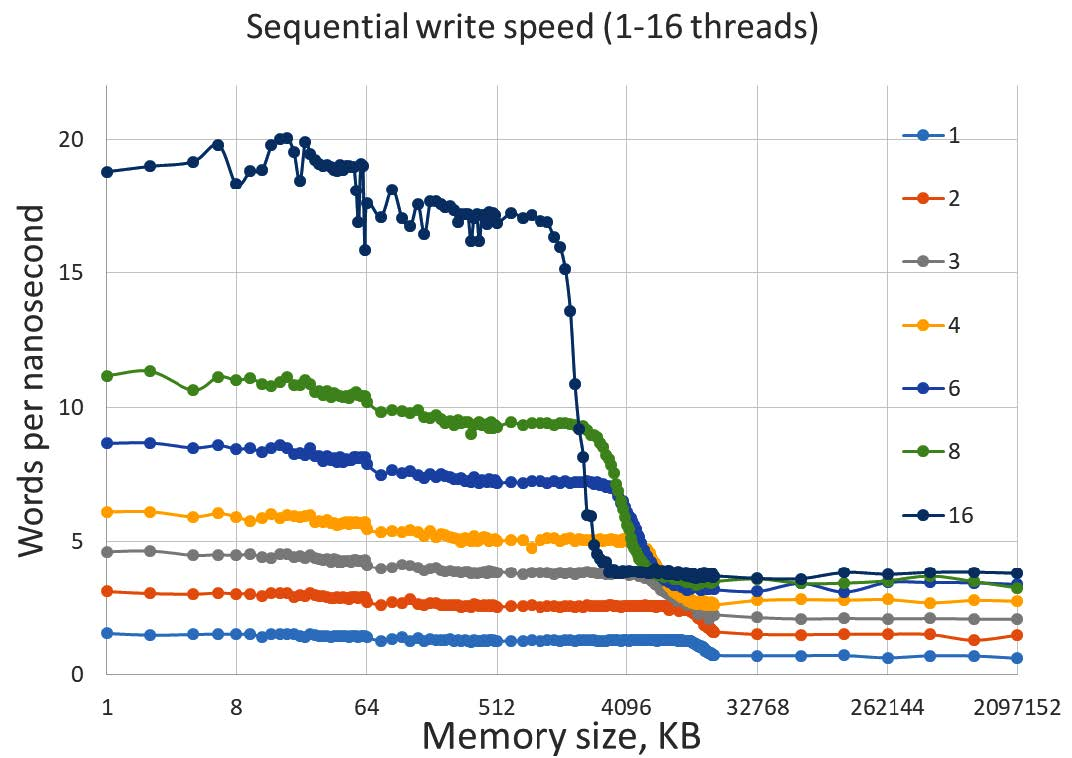
\includegraphics[width=0.9\textwidth]{content/1/chapter5/images/1.jpg}\\
圖5.1 - 連續寫入64位整數的內存吞吐量(每納秒字數),線程數的範圍為1到16
\end{center}

看到了與緩存大小相對應的速度。現在關注不同數量線程的曲線之間的差異,得到了從1到16個線程的結果(用於收集這些數據的機器確實至少有16個物理CPU核)。從圖的左邊開始,速度受到L1緩存(最多32KB)和L2緩存(256KB)的限制。處理器對每個核心都有單獨的L1和L2緩存,所以只要數據適合L2緩存,線程之間就沒有交互,因為它們不共享任何資源,每個線程都有自己的緩存。實際上,這並不完全正確,即使在較小的內存範圍內,也有CPU組件是共享的。不過,這個結論又幾乎是正確的。2個線程的吞吐量是1個線程的兩倍,4個線程寫入內存的速度又快了一倍,16個線程幾乎比4個線程快4倍。

當數據超過L2緩存的大小,進入L3緩存,然後進入主存時,情況發生了巨大的變化。這個系統中,L3緩存是在所有CPU內核之間共享的。主內存也是共享的,儘管不同的內存更接近於不同的CPU(非統一的內存架構)。對於1、2甚至4個線程,吞吐量繼續隨著線程數量的增加而增加,主內存似乎有足夠的帶寬,可以支持最多4個處理器的全速寫入。然後,當線程數從6增加到16時,吞吐量幾乎沒有增加。內存總線已經飽和了,不能更快地寫數據了。

如果這還不夠糟糕,請考慮這些結果是在撰寫本文時(2020年)在最新的硬件上獲得的。在2018年時,作者在他的課上展示的圖表:

%\hspace*{\fill} \\ %插入空行
\begin{center}
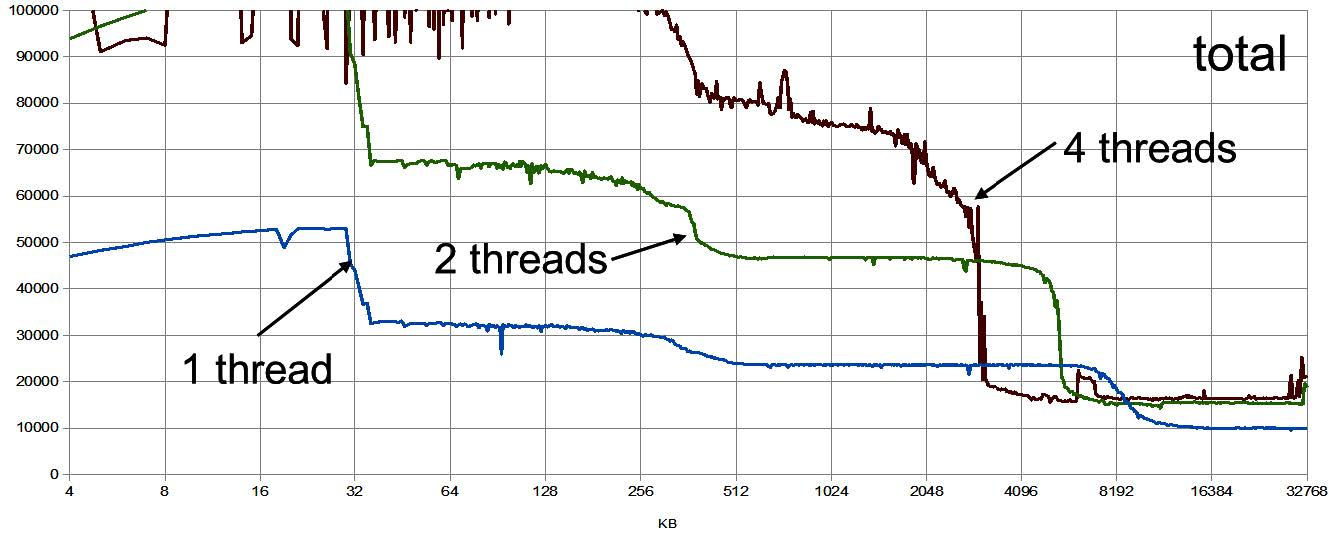
\includegraphics[width=0.8\textwidth]{content/1/chapter5/images/2.jpg}\\
圖5.2 -舊CPU(2018)的內存吞吐量
\end{center}

這個系統有一個內存總線,使用兩個線程就完全飽和了。讓我們看看這對併發程序的性能有什麼影響。

\subsubsubsection{5.2.4\hspace{0.2cm}內存受限和併發性}

同樣的結果可以用不同的方式來表示。通過繪製每個線程的內存速度(相對於一個線程),這裡專注於併發對內存速度的影響:

%\hspace*{\fill} \\ %插入空行
\begin{center}
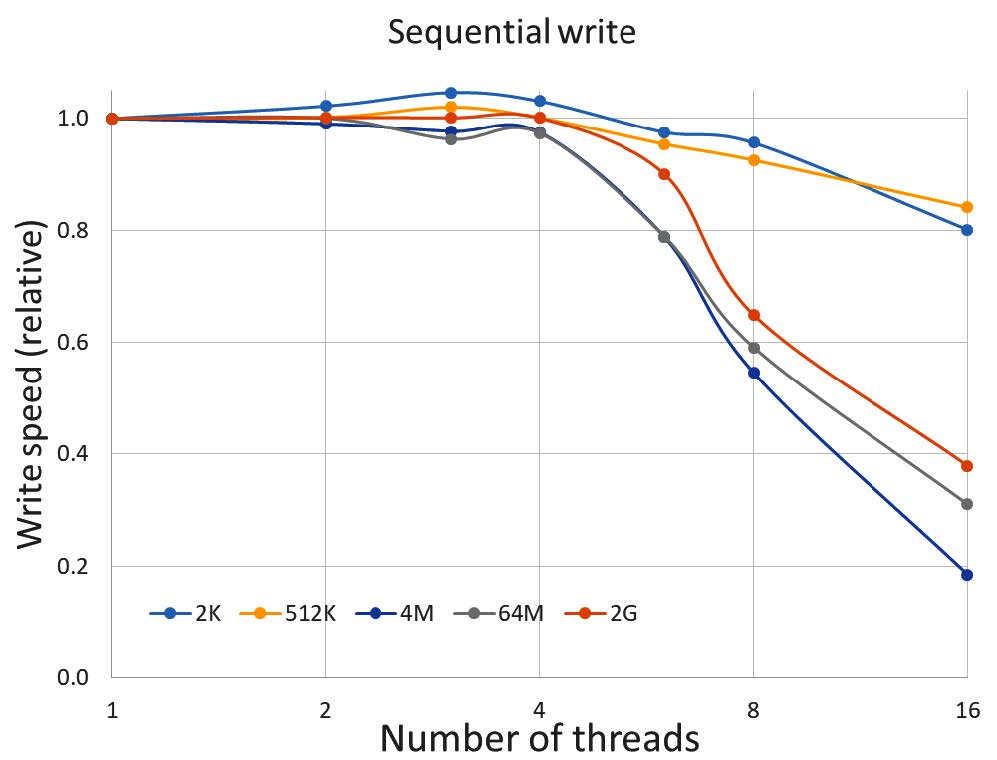
\includegraphics[width=0.7\textwidth]{content/1/chapter5/images/3.jpg}\\
圖5.3 - 內存吞吐量(相對於單個線程的吞吐量),以及線程數量
\end{center}

隨著內存速度的標準化,所以單線程總是1,對於適合L1或L2緩存的小數據集,每個線程的內存速度幾乎保持不變,即使是16個線程(每個線程的寫入速度是單線程速度的80\%)。然而,進入L3緩存或超過它的大小,4個線程之後速度就會下降。從8個線程增加到16個線程性能改進就非常小了。系統中沒有足夠的帶寬以足夠快的速度將數據寫入內存。

儘管用於讀取內存的帶寬通常比用於寫入的帶寬稍好一些,但不同內存訪問模式的結果看起來非常接近。

如果程序在單線程的情況下內存受限,那麼性能就會受到在主內存中移動數據速度的限制。可以期望從併發性中獲得的性能改進時,就要受到嚴格的限制。若這不適用於你,可能是因為你沒有一個16核處理器,廉價的處理器有廉價的內存總線,所以大多數4核系統也沒有足夠的內存帶寬給所有的核。

對於多線程程序,更重要的是要避免內存限制。這裡使用的技術是分割計算,這樣可以在更小的數據集上完成更多的工作,這些數據集適合存放於L1或L2緩存,再重新安排計算,這樣可以用更少的內存訪問完成更多的工作,通常會以重複一些計算為代價。優化內存訪問模式,這樣內存是順序訪問,而不是隨機訪問(即使可以飽和這兩種訪問模式,順序訪問的總帶寬要大得多,因此對於相同數量的數據,如果使用隨機訪問,程序可能會受到內存限制,而如果使用順序訪問,則完全不受內存速度的限制)。僅靠實現技術是不夠的,並且不能產生預期的性能改進,那麼下一步就是使算法適應併發編程。許多問題都有多個算法,並且其內存需求不同。對於單線程程序來說,最快的算法通常會被另一種更適合併發的算法所超越,在單線程執行速度上的損失,可以通過可擴展執行進行彌補。

目前為止,我們假設每個線程都獨立於所有其他線程完成自己的工作。由於對有限資源(如內存帶寬)的爭用,線程之間的唯一的交互是間接的。這是最容易編寫的程序,但大多數實際情況中的程序不允許這樣的限制。這帶來了一系列全新的性能問題,是時候來瞭解這些問題了。


















